\section{线性离散系统的分析方法}

\subsection{连续信号的采样与重构}

\subsubsection{连续信号的采样}

\begin{equation*}
    f(t) \xrightarrow{\text{采样}} f^*(t)
\end{equation*}

原连续信号为$f(t)$,采样后的离散信号为$f^*(t)$,满足

\begin{equation}
    f^*(t) = \sum_{k=0}^{\infty} f(kt) \delta(t-kT) = f(t)p(t)
\end{equation}

即理想采样信号$f^*(t)$可以看成连续信号$f(t)$和理想采样脉冲序列$\delta_{\rm T}(t)$的乘积。

理想采样:忽略脉冲宽度$\tau$,即瞬时采样。

\begin{theorem}[采样定理]
    连续信号采样后产生的高频幅频谱与基本幅频谱不发生重叠的条件是
    \begin{equation}
        (\text{采样频率}) \omega_s \geqslant 2 \omega_c (\text{连续信号最高频率})
    \end{equation}
\end{theorem}

\subsubsection{采样信号的重构}

重构条件:
\begin{enumerate}
    \item 满足采样定理;
    \item 采用理想滤波器。
\end{enumerate}
重构的实质是把一串脉冲序列$f(0)$,$f(T)$,$\cdots$,$f(kT)$平滑成连续的信号$f(t)$,常用Taylor级数多项式外推。

\subsubsection{零阶保持器}

\begin{equation}
    f_k(t) = f(kT),\,kT \leqslant t < (k+1)T
\end{equation}

零阶保持器将$f^*(t)$在$kT$时的状态保持到$(k+1)T$到来之前,其传递函数为

\begin{equation}
    G_{H_0}(s) = \frac{1-{\rm{e}}^{-Ts}}{s}
\end{equation}

\subsection{$Z$变换与反$Z$变换}

$f(t)$的$Z$变换和$f^*(t)$的$Z$变换结果相同,即

\begin{equation}
    \Z{f(t)} = \Z{f^*(t)} = F(z) = \sum_{k=0}^{\infty} f(kT) z^{-k}
\end{equation}

反过来,\highlight{gray}{$F(z)$的反$Z$变换只能得到唯一的$f^*(t)$,但不能得到唯一的$f(t)$},即

\begin{equation}
    \ZF{F(z)} = f^*(t) = f(kT)
\end{equation}

此处涉及的计算需要多做习题,提高熟练度,也需要复习一下拉普拉斯变换的知识。

\subsubsection{$Z$变换的计算}

\begin{align}
    & F(z) = \sum_{i=1}^{n} \lim_{s\to s_i} (s - s_i)\frac{F(s) z}{z - {\rm{e}}^{Ts}} \\
    & F(z) = \sum_{i=1}^{n} \lim_{s\to s_i} \frac{1}{(m_i - 1)!} \dvn{m_i-1}{s} \left[(s-s_i)^{m_i} \frac{F(s) z}{z - {\rm{e}}^{Ts}}\right]
\end{align}

\subsubsection{$Z$反变换的计算}

\begin{align}
    & f(k) = \sum_{i=1}^{n} \lim_{z\to z_i} (z - z_i) F(z) z^{k-1} \quad k=1, 2, 3, \cdots \\
    & f(k) = \sum_{i=1}^{n} \lim_{z\to z_i} \frac{1}{(m_i - 1)!} \dvn{m_i-1}{z} \left[(z-z_i)^{m_i} F(z) z^{k-1}\right] \quad k=1, 2, 3, \cdots 
\end{align}

\subsubsection{$Z$变换求解差分方程}

对差分方程两边同时作$Z$变换,解出$Y(z)$后,求其$Z$反变换。

此处常用以下两个性质,并注意此时$T=1\,{\rm s}$

\begin{align}
    & \Z{f(t+nT)} = z^n F(z) - \sum_{j=0}^{n-1} z^{n-j} f(j) \\
    & \Z{\delta(k)} = 1
\end{align}

\subsection{线性离散系统的脉冲传递函数}

\begin{definition}[脉冲传递函数]
    在零初始条件下,一个环节或系统的输出序列$Z$变换与输入序列$Z$变换之比,用
    \begin{equation}
        G(z) = \frac{C(z)}{R(z)}
    \end{equation}
    来表示。
\end{definition}

线性离散系统的脉冲传递函数只与系统本身的结构参数与性能有关,\highlight{\gray}{与输入信号无关。}

\begin{enumerate}
    \item 系统含有保持器时
    \begin{equation}
        G(z) = \Z{G(s) G_H(s)}
    \end{equation}
    \item 串联环节
    \begin{figure}[H]
        \centering
        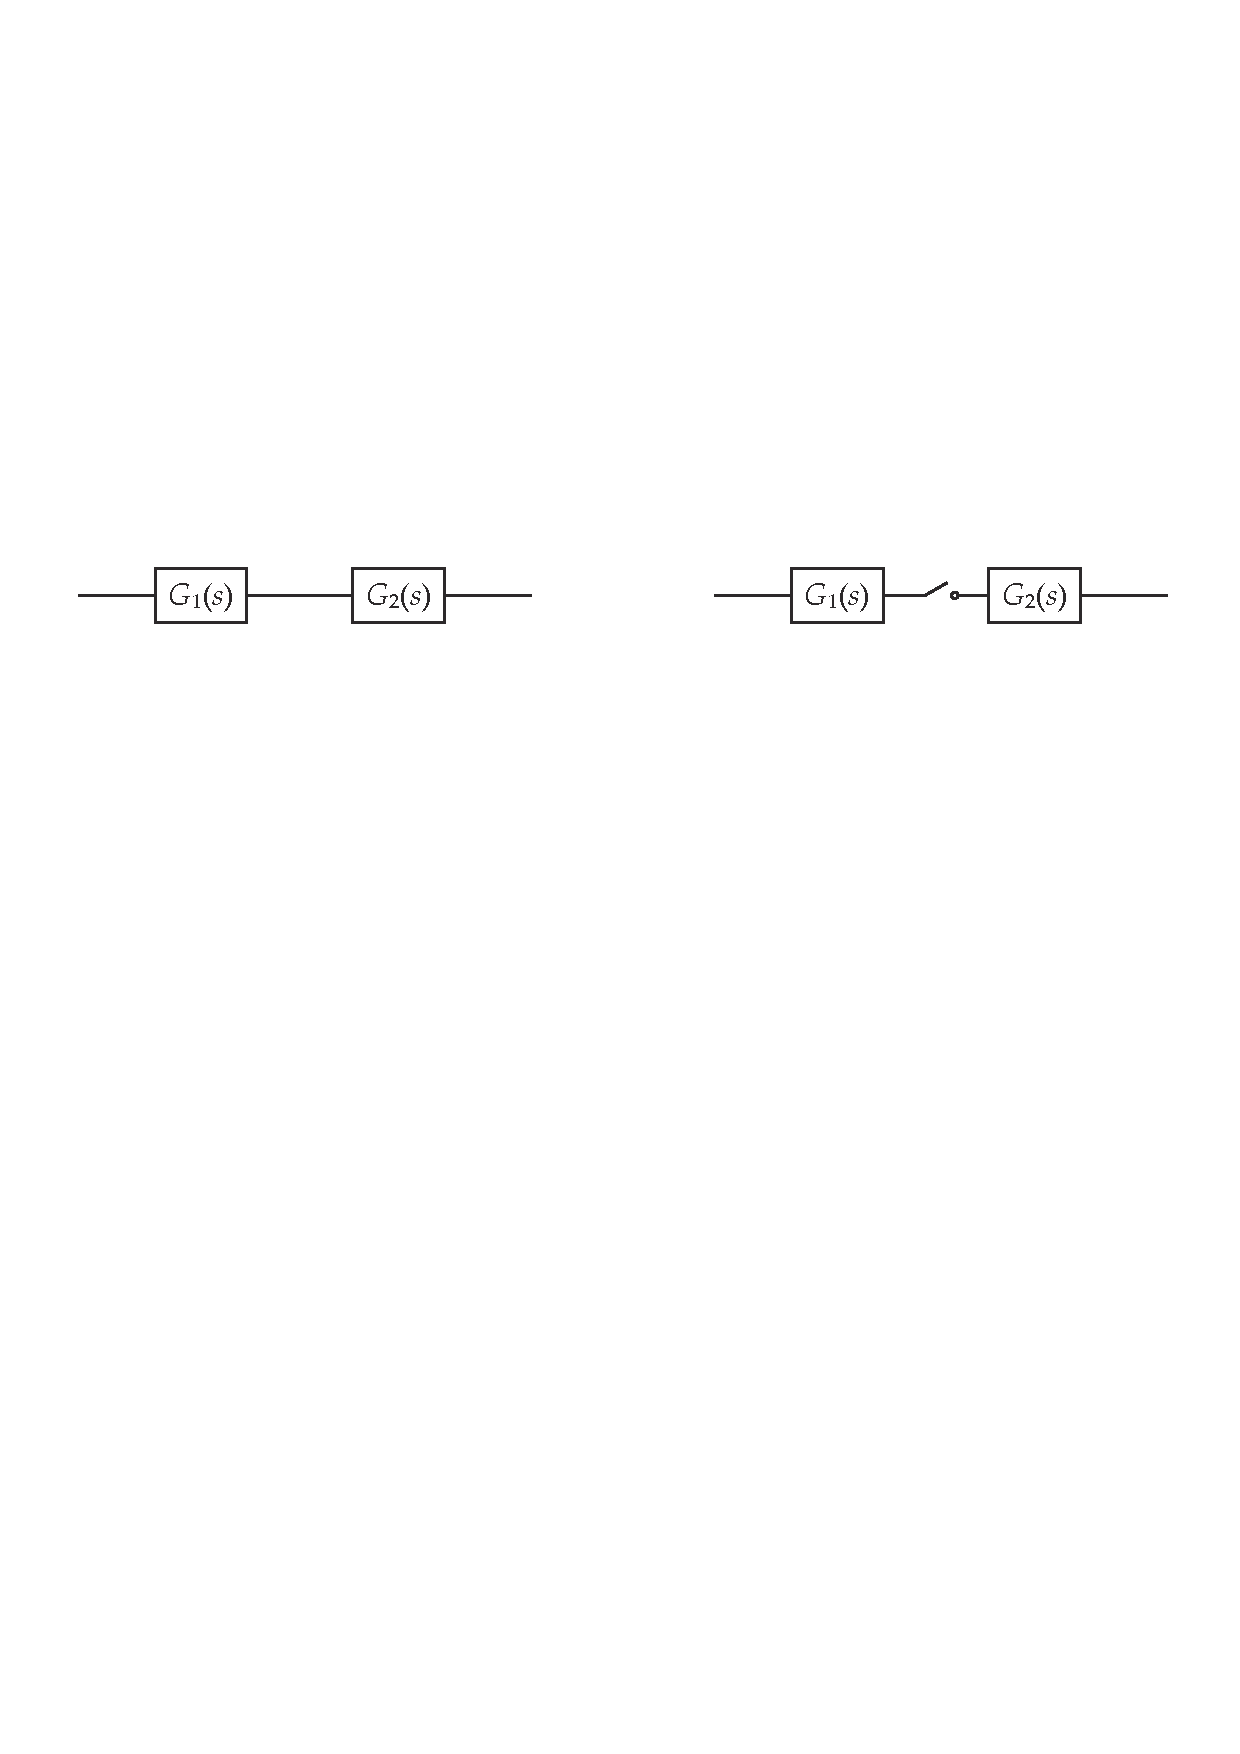
\includegraphics[scale=0.7]{figures/figure2.1.pdf}
    \end{figure}

    \begin{multicols}{2}
        \begin{equation}
            G(z) = \Z{G_1(s) G_2(s)}
        \end{equation}

        \begin{equation}
            G(z) = \Z{G_1(s)} \Z{G_2(s)}
        \end{equation}
    \end{multicols}
    \item 闭环脉冲传递函数
    此处注意对例2-12种$Z$变换过程的理解。
    \begin{figure}[H]
        \centering
        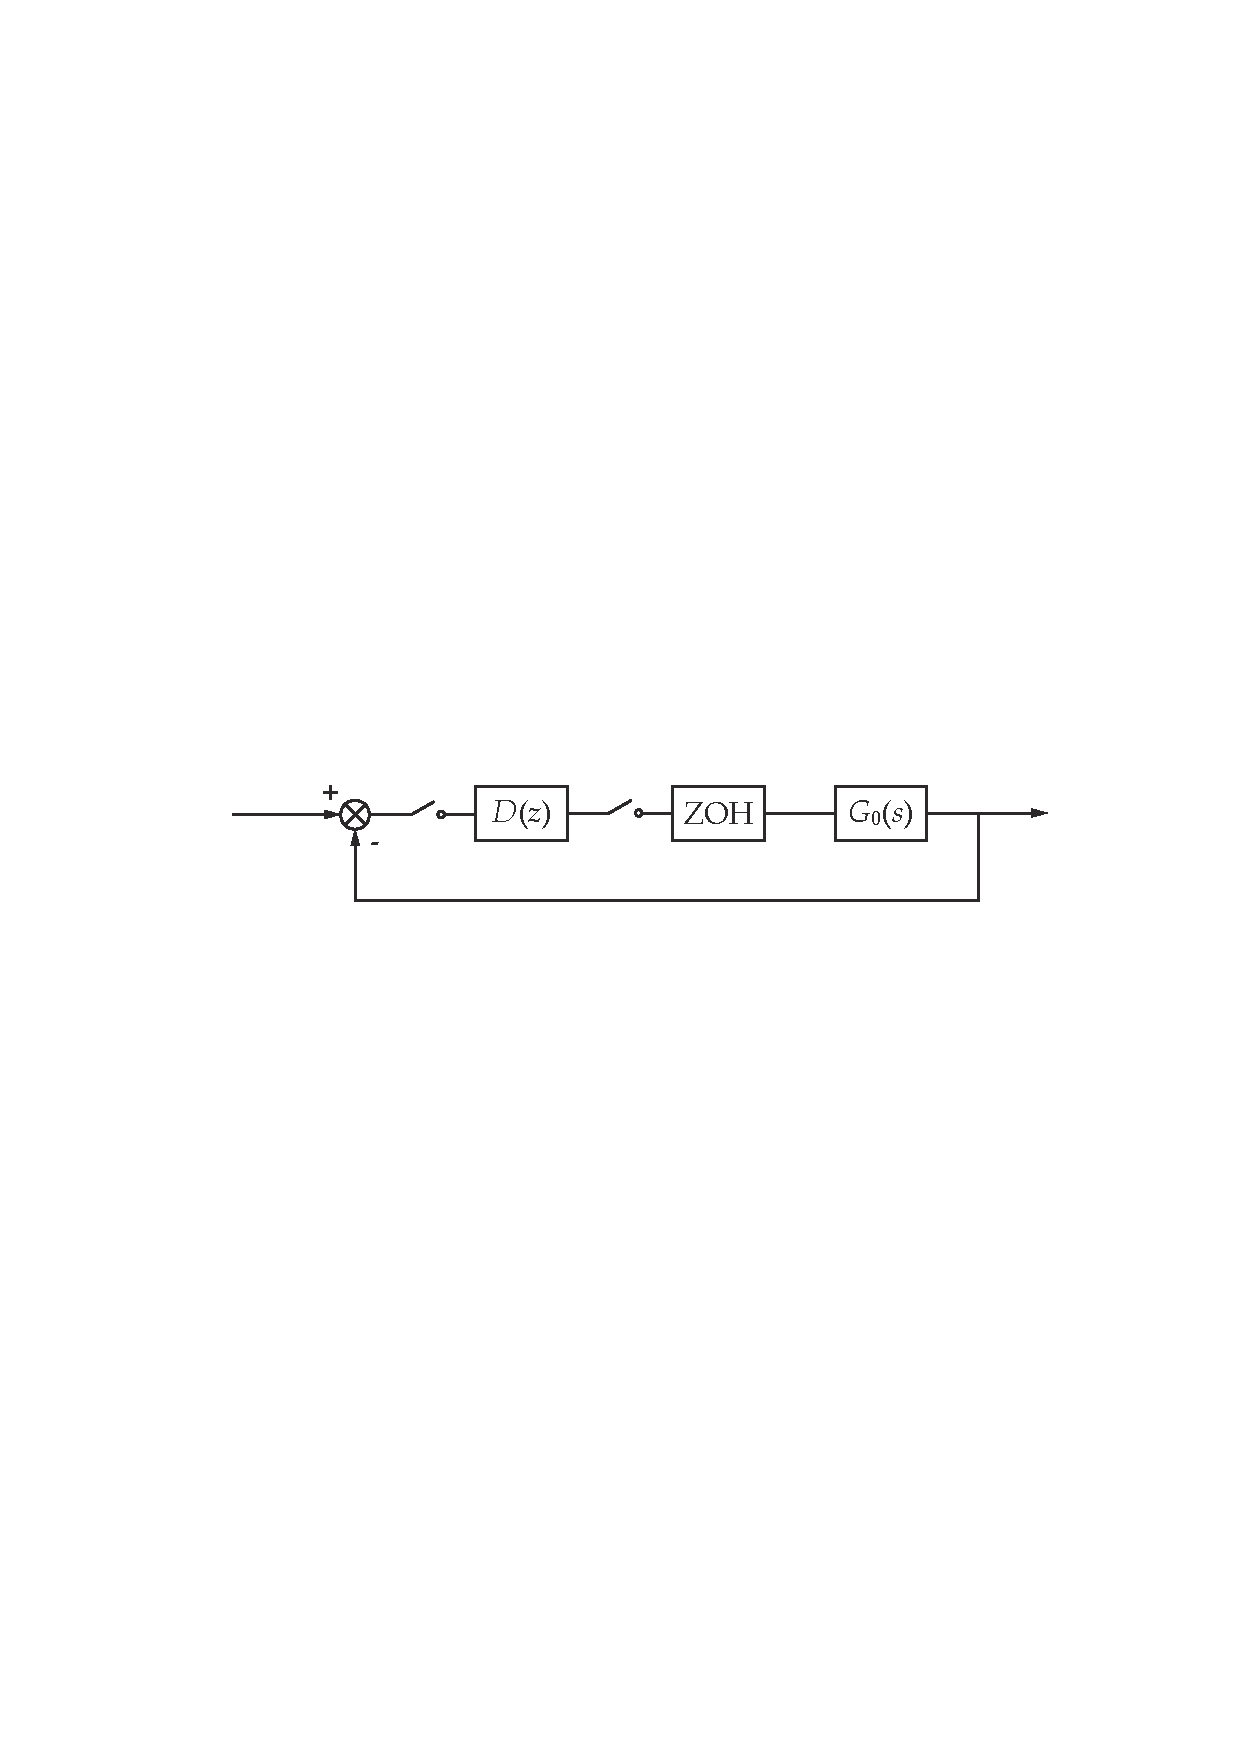
\includegraphics[scale=0.7]{figures/figure2.2.pdf}
    \end{figure}
    \begin{align}
        & G(z) = \Z{G(s)} = \Z{G_{H_0}(s) G_0(s)} \\
        & W(z) = \frac{C(z)}{R(z)} = \frac{D(z) G(z)}{1 + D(z)G(z)}
    \end{align}
\end{enumerate}

\subsection{习题选解}

\begin{exercise} % 2.3
    \begin{enumerate}
        \item \begin{align*}
            F(s)&= \mathcal{L}\left[f(t)\right] = \frac{1}{s+2a} \\
            F(z)&= \Z{F(z)} = \lim_{s \to -2a} (s+2a) \frac{z}{(s+2a)(z-{\rm e}^{Ts})} = \frac{z}{z-{\rm e}^{-2aT}}
        \end{align*}
        \item \begin{align*}
            F(s)&= \mathcal{L}\left[f(t)\right] = \frac{3}{s^2} \\
            F(z)&= \Z{F(s)} = \lim_{s \to 0} \frac{1}{(2-1)!} \dvn{}{s} \left[s^2 \cdot \frac{3z}{s^2 (z - {\rm e}^{Ts})}\right] = \lim_{s \to 0} \frac{3z T{\rm e}^{Ts}}{(z-{\rm e}^{Ts})^2} = \frac{3zT}{(z-1)^2}
        \end{align*}
        \item \begin{align*}
            F(s) = \mathcal{L}\left[f(t)\right] &= \frac{2}{(s+1)^2 + 4} \\
            F(z) = \Z{F(s)} &= \lim_{s \to -1-2j} (s+1+2j)\cdot \frac{2z}{[(s+1)^2+4] (z-{\rm e}^{Ts})} + \lim_{s \to -1+2j} (s+1-2j)\cdot \frac{2z}{[(s+1)^2+4] (z-{\rm e}^{Ts})} \\
                &= \lim_{s \to -1-2j} \frac{2}{s+1-2j} \cdot \frac{z}{z-{\rm e}^{Ts}} + \lim_{s \to -1+2j} \frac{2}{s+1+2j} \cdot \frac{z}{z-{\rm e}^{Ts}} \\
                &= \frac{1}{2j} \left[\frac{z}{z-{\rm e}^{(-1+2j)T}} - \frac{z}{z-{\rm e}^{-(1+2j)T}}\right]
        \end{align*}
        \item \begin{align*}
            F(z) = \Z{F(s)} &= \lim_{s \to -1} \frac{s+3}{s+2} \cdot \frac{z}{z-{\rm e}^{Ts}} + \lim_{s \to -2} \frac{s+3}{s+1} \cdot \frac{z}{z-{\rm e}^{Ts}} \\
            &= \frac{2z}{z-{\rm e}^{-T}} - \frac{z}{z-{\rm e}^{-2T}}
        \end{align*}
        \item \begin{align*}
            F(z) = \Z{F(s)} &= \lim_{s \to 0} \frac{1}{s^2+1} \cdot \frac{z}{z-{\rm e}^{Ts}} + \lim_{s \to -j} \frac{1}{s(s-j)} \cdot \frac{z}{z-{\rm e}^{Ts}} + \lim_{s \to j} \frac{1}{s(s+j)} \cdot \frac{z}{z-{\rm e}^{Ts}} \\
            &= \frac{z}{z-1} - \frac{z}{2(z-{\rm e}^{-jT})} - \frac{z}{2(z-{\rm e}^{jT})}
        \end{align*}
    \end{enumerate}
\end{exercise}

\begin{exercise} % 2.4
    \begin{enumerate}
        \item \begin{align*}
            F(s) = \ZF{F(z)} &= \lim_{z \to -1} \frac{z}{z-1} \cdot z^{k-1} + \lim_{z \to 1} \frac{z}{z+1} \cdot z^{k-1} \\
            &= \frac{1-(-1)^k}{2} \quad k = 1, 2, \cdots
        \end{align*}
        \item \begin{align*}
            F(s) = \ZF{F(z)} &= \lim_{z \to 1} \frac{1}{(2-1)!} \dvn{}{z} \left(\frac{z}{z-2} \cdot z^{k-1}\right) + \lim_{z \to 2} \frac{z}{(z-1)^2} \cdot z^{k-1} \\
            &= 2^k - k - 1 \quad k = 1, 2, \cdots
        \end{align*}
        \item \begin{equation*}
            F(s) = \ZF{F(z)} = \lim_{z \to 0} \frac{z^{k-1}}{z-0.2} + \lim_{z \to 0.2} \frac{z^{k-1}}{z} = 0.2^{k-2} \quad k = 1, 2, \cdots
        \end{equation*}
    \end{enumerate}
\end{exercise}

\begin{exercise} % 2.5
    此题差分方程应为
    \begin{enumerate}
        \item $y(k+2) - 5y(k+1) + 6y(k) = 0,\, y(0) = 0,\, y(1) = 1$
        \item $y(k+2) - 2y(k+1) + y(k) = k,\, y(0) = 0,\,y(1) = 0$
    \end{enumerate}

    \begin{enumerate}
        \item 两边同时$Z$变换,得
        \begin{equation*}
            z^2 Y(z) - z^2 y(0) - z y(1) - 5[z Y(z) - zy(0)] + 6Y(z) = 0
        \end{equation*}
        化简,得
        \begin{equation*}
            z^2 Y(z) - z - 5z Y(z) + 6Y(z) = 0
        \end{equation*}
        解得
        \begin{equation*}
            Y(z) = \frac{z}{(z-2)(z-3)}
        \end{equation*}
        做$Z$反变换,得
        \begin{align*}
            y(k) = \ZF{Y(z)} &= \lim_{z \to 2} \frac{z}{z-3} \cdot z^{k-1} + \lim_{z \to 3} \frac{z}{z-2} \cdot z^{k-1} \\
            &= 3^k - 2^k \quad k = 1, 2, \cdots
        \end{align*}
        \item 两边同时$Z$变换,得(此处$T=1\,{\rm s}$)
        \begin{equation*}
            z^2 Y(z) - z^2 y(0) - z y(1) - 2[z Y(z) - zy(0)] + Y(z) = \frac{z^{-1}}{(1-z^{-1})^2}
        \end{equation*}
        化简,得
        \begin{equation*}
            z^2 Y(z) - 2z Y(z) + Y(z) = \frac{z}{(z-1)^2}
        \end{equation*}
        解得
        \begin{equation*}
            Y(z) = \frac{z}{(z-1)^4}
        \end{equation*}
        做$Z$反变换,得
        \begin{align*}
            y(k) = \ZF{Y(z)} &= \lim_{z \to 1} \frac{1}{(4-1)!} \cdot \dvn{3}{z} \left(z\cdot z^{k-1}\right) \\
            &= \frac{k(k-1)(k-2)}{6} \quad k = 1, 2, \cdots
        \end{align*}
    \end{enumerate}
\end{exercise}
